\documentclass[12pt]{article}

\usepackage[letterpaper]{geometry}
\geometry{
	left=20mm,
	right=20mm,
}

\usepackage{enumitem}
\usepackage{hyperref}
\usepackage{graphicx}
\usepackage{wrapfig}
\usepackage{float}

\graphicspath{ {./images/} }

\begin{document}
\begin{titlepage}
	\begin{center}
		\vspace*{1cm}

		\Huge
		\textbf{Week 5 Lab Report}

		\vspace{0.2cm}
		\LARGE
		CPS 706 Computer Networks

		\vspace{1.5cm}

		\textbf{Mitchell Mohorovich}\\
		\vspace{0.2cm}
		\Large
		500563037\\
		\Large
		Section 5, Fridays 2-3PM

		\vfill

		\vspace{0.8cm}

		\Large
		Computer Science\\
		Ryerson University\\
	\end{center}
\end{titlepage}

\section{nslookup}
\begin{enumerate}
	\item{\textit{Run nslookup to obtain the IP address of a Web server in Asia.}}\\ \\
		I used nslookup to find the IP address of \url{google.jp}, it returned \url{172.217.22.99}. 

		\begin{figure}[H]
			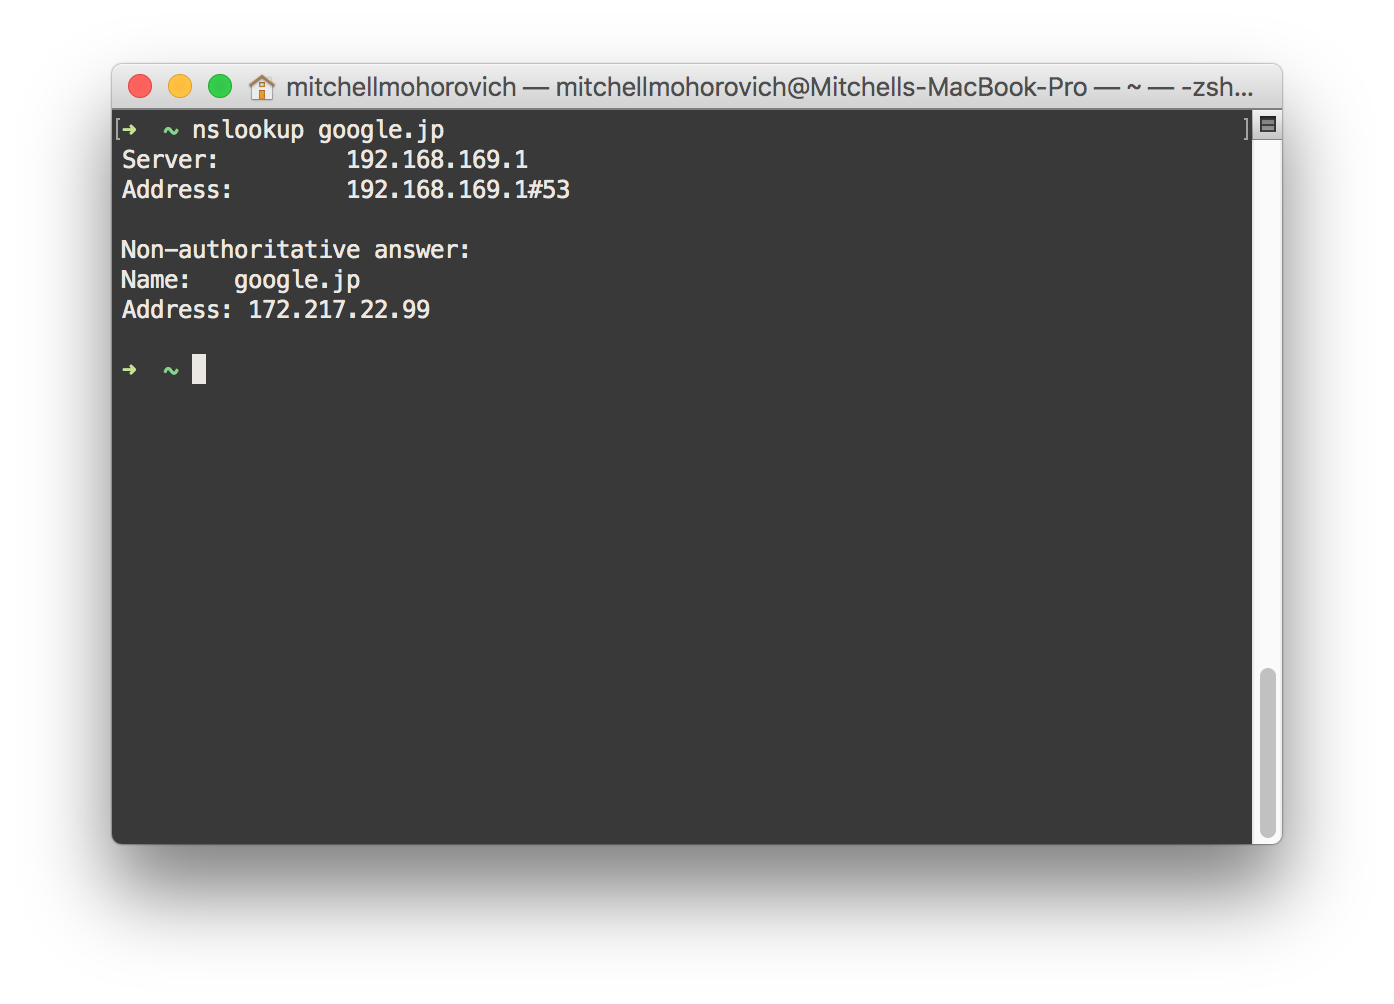
\includegraphics[width=1\textwidth]{google_japan}%
			\caption{Using nslookup to find the IP of Google Japan}
		\end{figure}

	\item{\textit{Run nslookup to determine the authoritative DNS servers for a university in Europe.}}\\ \\
		I used nslookup to find the name servers for the University of Florence. The results are shown in Figure 2 below.

		\begin{figure}[H]
			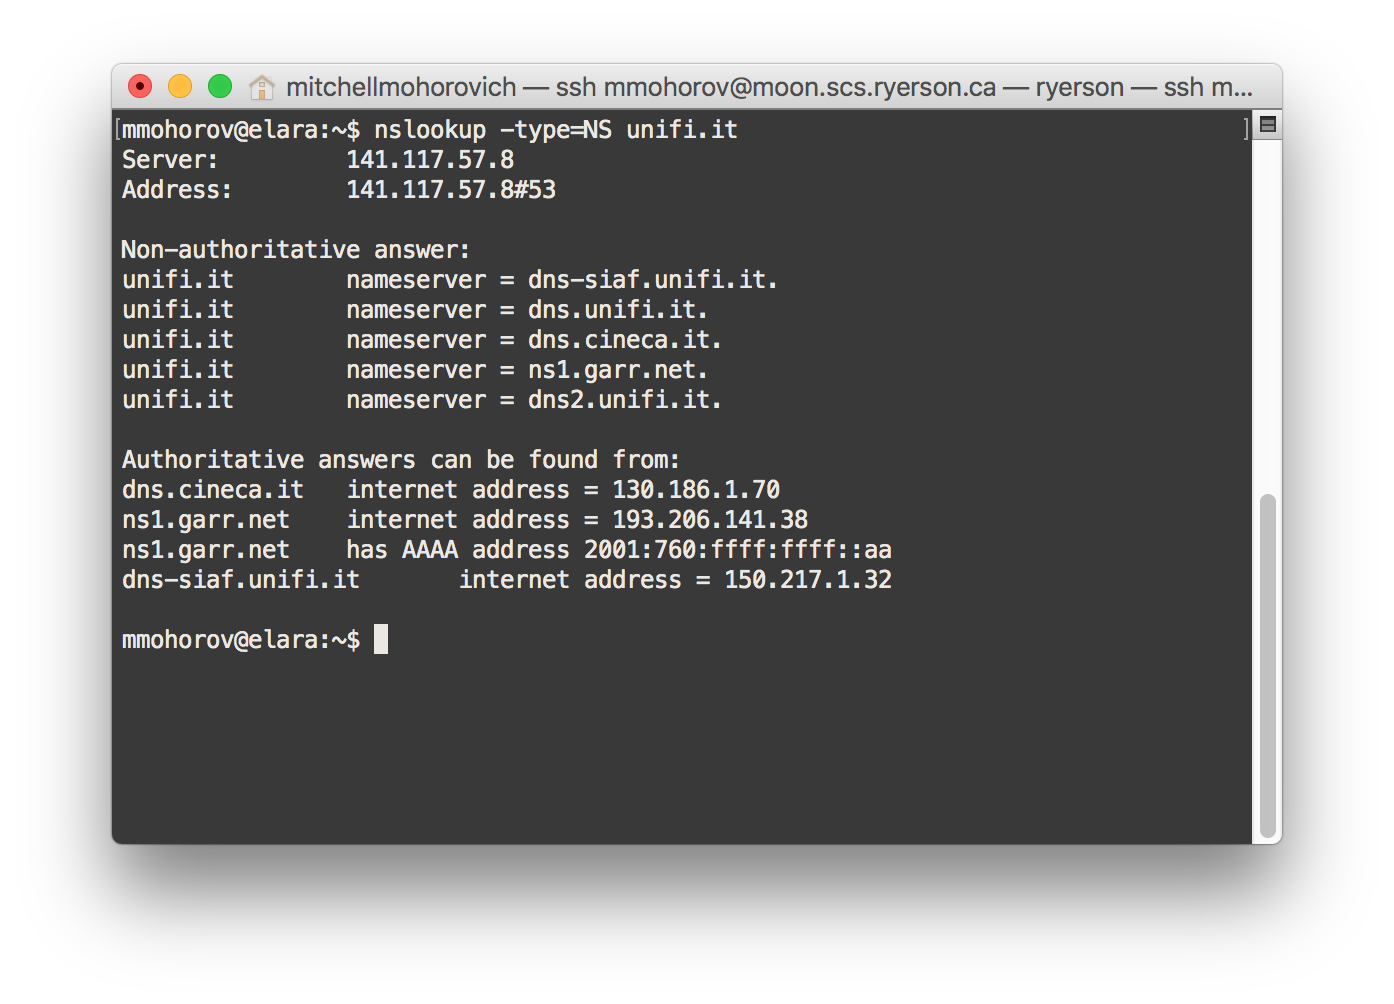
\includegraphics[width=1\textwidth]{florence_university}%
			\caption{Using nslookup to find the name servers of the University of Florence}
		\end{figure}

	\item{\textit{Run nslookup so that one of the DNS servers obtained in Question 2 is queried for the mail servers for Yahoo! mail.}}\\ \\
		I was unable to find a DNS server run by a European university that would allow for external queries, so I used the OpenDNS public DNS server to complete this part of the lab. The screenshot of the command is shown in the screenshot below.

		\begin{figure}[H]
			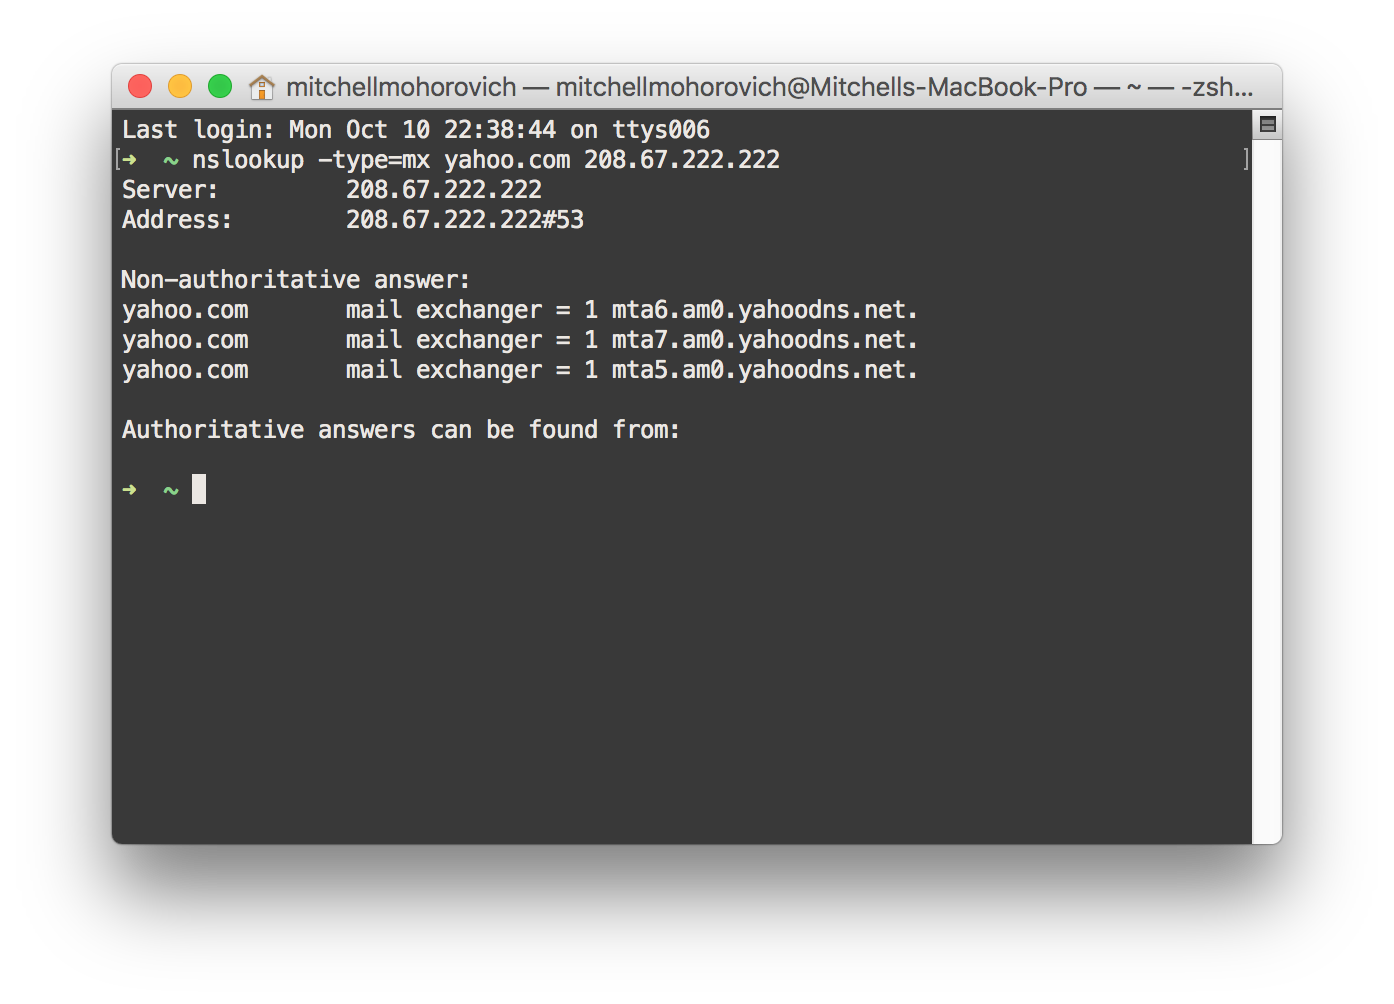
\includegraphics[width=1\textwidth,center]{google_dns}%
			\caption{Using nslookup to use OpenDNS Public DNS to return a query to find the mail servers of Yahoo!}
		\end{figure}

\end{enumerate}


\section{Tracing DNS with Wireshark}
\begin{enumerate}
		\setcounter{enumi}{3}
	\item{\textit{Locate the DNS query and response messages. Are they sent over UDP or TCP?}}\\ \\
		The DNS query and response messages are send over UDP. This is shown by the protocol flag in the packet.

	\item{ \textit{What is the destination port for the DNS query message? What is the source port of DNS response message?} }\\ \\
		The destination port for the DNS query message is 53. The source port of the response message is 53 as well.

	\item{\textit{To what IP address is the DNS query message sent? Use ipconfig to determine the IP address of your local DNS server. Are these two IP addresses the same?}}\\ \\
		The query message is sent to \url{8.8.8.8}. This IP is the same as my local DNS server, which is \url{8.8.8.8}. This is because I have my DNS server manually set to Google's DNS server at \url{8.8.8.8}.

	\item{\textit{Examine the DNS query message. What “Type” of DNS query is it? Does the query message contain any ``answers''?}}\\ \\
		Based on the DNS flags provided in the query packet, a standard DNS query was sent. The query contains three ``answers''.

	\item{\textit{Examine the DNS response message. How many “answers” are provided? What do each of these answers contain?}}\\ \\
		There are three ``answers'' provided, one is a CNAME DNS record, and the other two are A records. The first CNAME record says that the domain \url{www.ietf.org maps} maps to \url{www.ietf.org.cdn.cloudflare-dnssec.net}. The other two A records return two separate IP addresses for the URL in the CNAME record, one IP used as a primary IP address, the other as a backup (presumably) for the CDN.
 
	\item{\textit{Consider the subsequent TCP SYN packet sent by your host. Does the destination IP address of the SYN packet correspond to any of the IP addresses provided in the DNS response message?}}\\ \\
		The IP address subsequent TCP SYN packet sent by my host corresponds to the IP address of the first A record received.

	\item{\textit{This web page contains images. Before retrieving each image, does your host issue new DNS queries?}}\\ \\
		No, my host did not issue new DNS queries. Since the images were hosted on the same domain and the DNS records retrieved had a TTL of 244, my host used the cached records stored locally.
		
	\item{\textit{What is the destination port for the DNS query message? What is the source port of DNS response message?}} \\ \\
		The destination port for the DNS query message is 53, the source port is 53 as well.

	\item{\texit{To what IP address is the DNS query message sent? Is this the IP address of your default local DNS server?} }\\ \\
		The DNS query message was sent to 8.8.8.8, this is the IP address of my default set local DNS server.

	\item{\textit{Examine the DNS query message. What “Type” of DNS query is it? Does the query message contain any “answers”?}}\\ \\ 
		The DNS query sent was a ``standard'' DNS query.

	\item{\textit{Examine the DNS response message. How many “answers” are provided? What do each of these answers contain?}}\\ \\
		The DNS query provides one answer. This answer is an A record that provides the IP address of the queried URL.

	\item{\textit{Provide a screenshot.}}
		\begin{figure}[H]
			\centering
			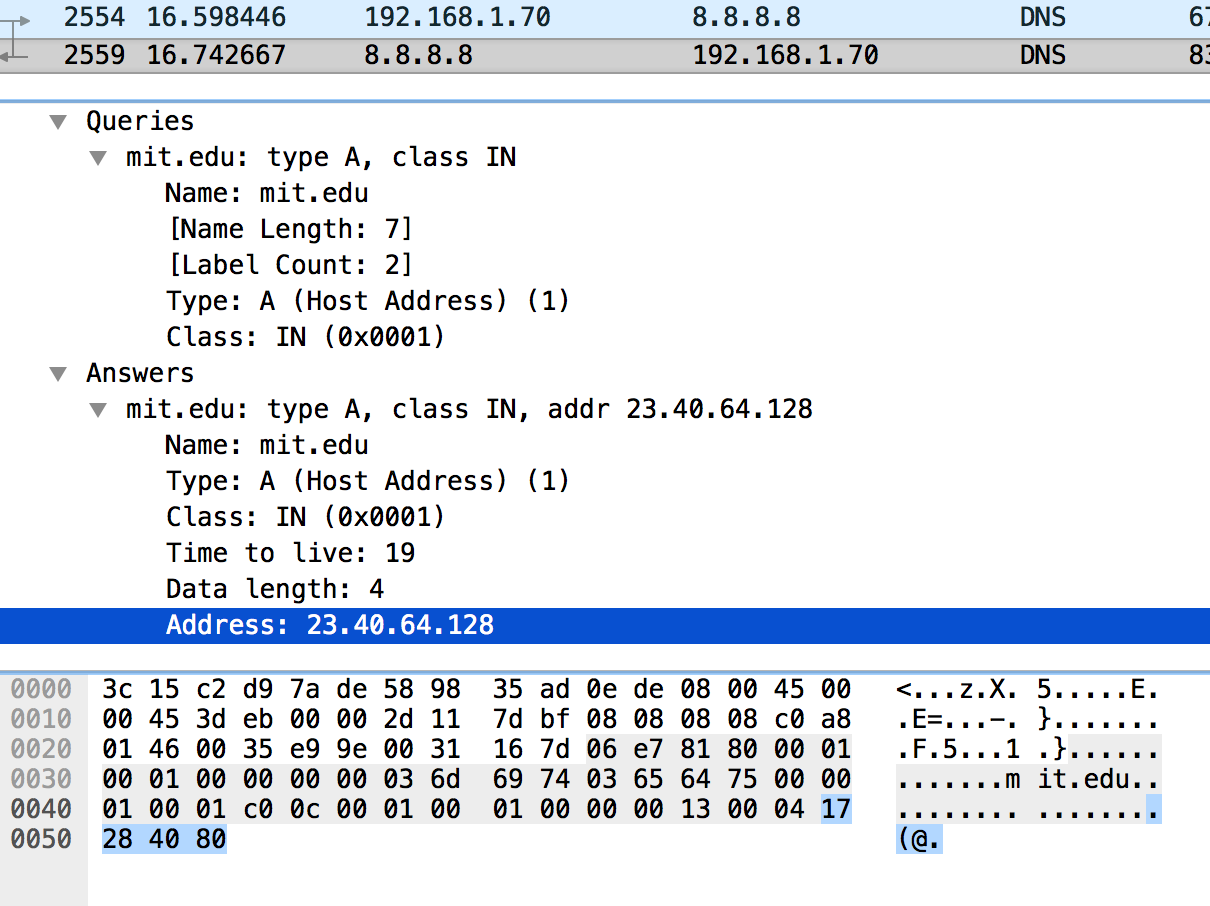
\includegraphics[width=0.80\textwidth,center]{15}%
			\caption{Screenshot of the answers returned from the nslookup command issued on \url{mit.edu}}
		\end{figure}

	\item{\textit{To what IP address is the DNS query message sent? Is this the IP address of your default local DNS server?}}\\ \\ 
		To DNS query message was sent to \url{8.8.8.8}, this is the IP address of my default local DNS server.

	\item{\textit{Examine the DNS query message. What “Type” of DNS query is it? Does the query message contain any “answers”?}}\\ \\
		The ``type'' of the DNS query is a standard query specified by the Flags of the DNS portion of the packet.

	\item{\textit{Examine the DNS response message. What MIT nameservers does the response message provide? Does this response message also provide the IP addresses of the MIT nameservers?}}\\ \\
		The DNS response message provides the answers to the query request, which were the nameservers for the \url{mit.edu} domain. The response message did not provide the IP addresses, but the domains of them.
	\item{\textit{Provide a screenshot.}}\\ \\ 
		\begin{figure}[H]
			\centering
			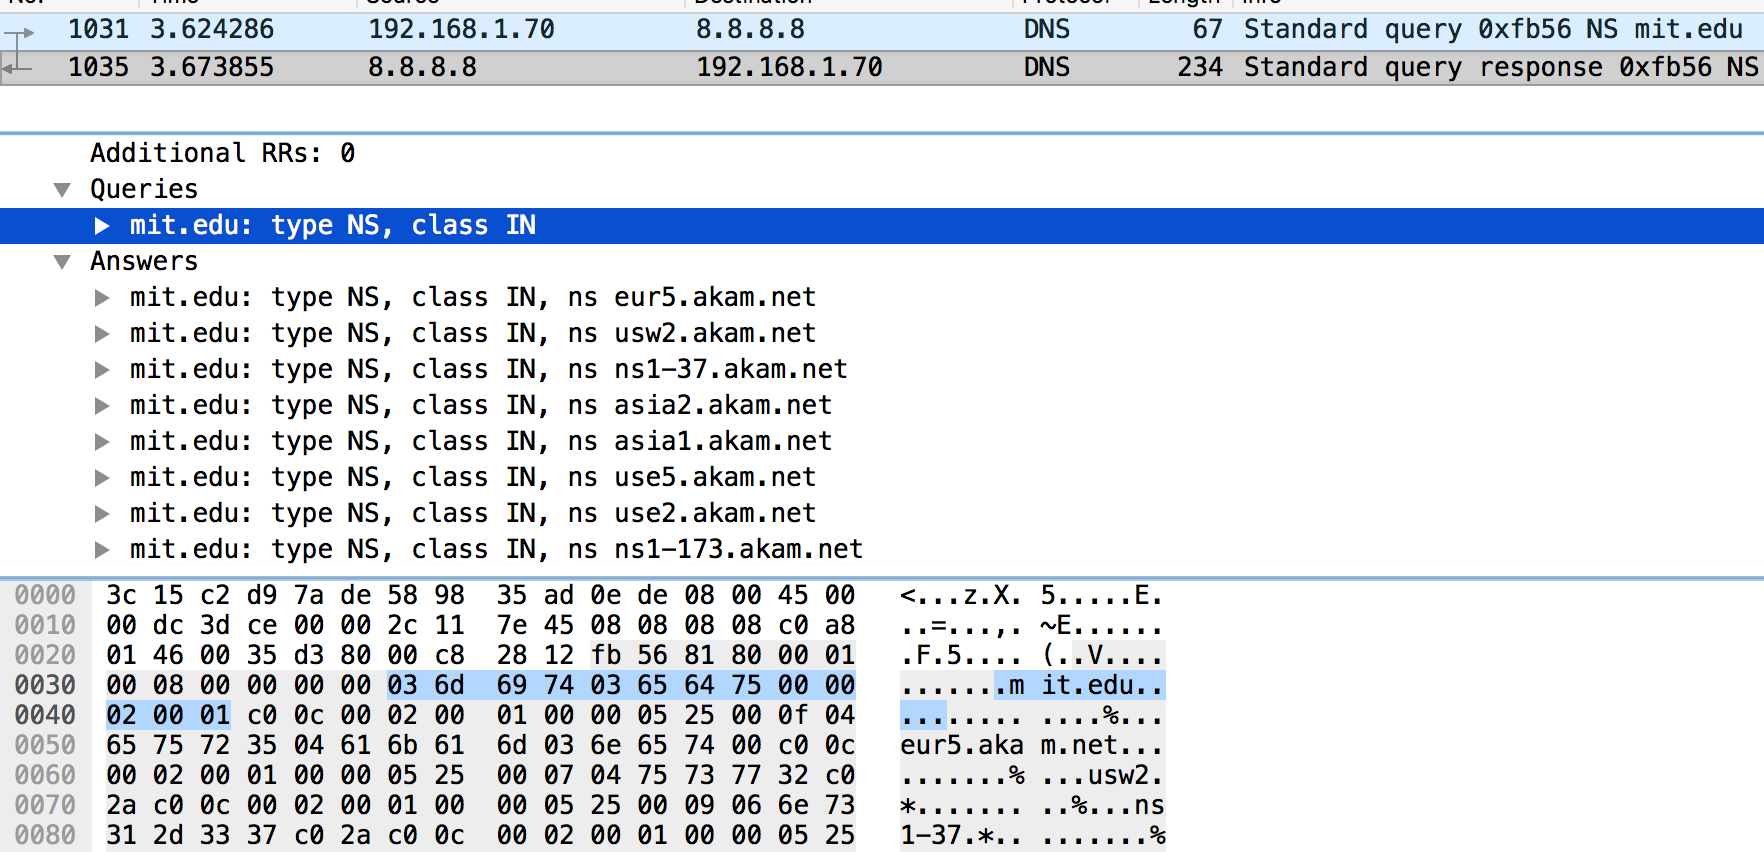
\includegraphics[width=1.0\textwidth]{19}%
			\caption{Screenshot of the answers returned from the nslookup command issued on \url{mit.edu}, requesting ns records}
		\end{figure}

		\textbf{Note: }\textit{For the following questions, instead of using \url{bitsy.mit.edu}, I used \url{resolver.opendns.com} as the DNS server to be queried, since \url{bitsy.mit.edu} was not working.}
 
	\item{\textit{To what IP address is the DNS query message sent? Is this the IP address of your default local DNS server? If not, what does the IP address correspond to?}}\\ \\
		The DNS query message was sent to \url{208.67.222.222}, which is the IP that the URL \url{resolver1.opendns.com} corresponds to.

	\item{\textit{Examine the DNS query message. What “Type” of DNS query is it? Does the query message contain any “answers”?}}\\ \\
		The DNS query message sent was a standard query.


	\item{\textit{Examine the DNS response message. How many “answers” are provided? What does each of these answers contain?}}\\ \\
		The DNS response message only contained one message. This one answer was an A record which maps the IP address \url{49.238.167.109} to the URL \url{www.aiit.or.kr}.


	\item{\textit{Provide a screenshot.}}\\ \\
		\begin{figure}[H]
			\centering
			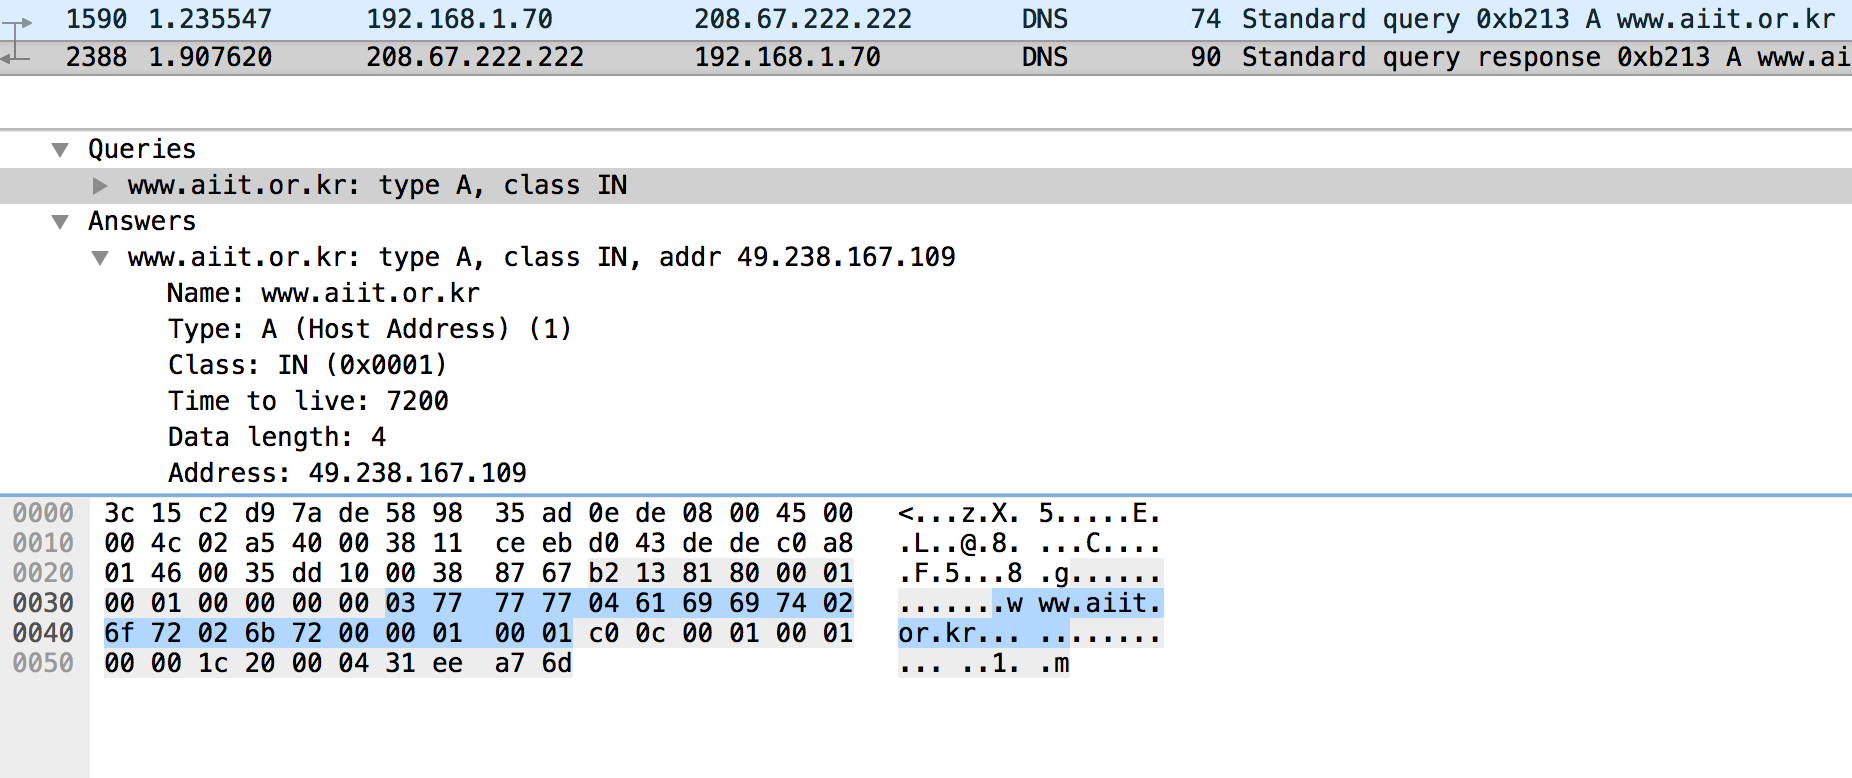
\includegraphics[width=1\textwidth]{23}%
			\caption{Screenshot of the answers returned from the nslookup command issued on \url{mit.edu}, with the -type=ns flag set to request for nameserver records}
		\end{figure}

\end{enumerate}


\end{document}
